\documentclass[hyperref={pdfpagelabels=false}, color=table]{beamer}
\usetheme{Madrid}
\useoutertheme[subsection=true]{miniframes}
\usepackage{lmodern}
\usepackage{tikz}
\usepackage{booktabs}
\usepackage{bookmark}
%\usepackage[usenames,dvipsnames]{color}
\usepackage{pgffor}
\usepackage{csvsimple}
\usepackage{hyperref}
\usepackage{colortbl}
\usepackage[first=0,last=9]{lcg}
\definecolor{LightCyan}{rgb}{0.88,1,1}
\newcommand{\ra}{\rand0.\arabic{rand}}
\usepackage{graphicx}
\usepackage{color}
\usetheme{Madrid}
\title{Corsound Interview Practical Test}
\author{Mor Zahavi}
\date{Corsound AI}
\begin{document}
    \logo{
\includegraphics[scale=0.14]{images/logo}}
    %   \logo{\includegraphics‏[scale=0.14]{figures/logo}}
    \begin{frame}
        \titlepage
    \end{frame}
    \begin{frame}\frametitle{Table of contents}
    \tableofcontents
    \end{frame}
    \section{Introduction}
    \subsection{Motivation}
    \begin{frame}
        \begin{itemize}
            \item The goal is to fit a classifier to distinguish real speech from fake.
            \item A solution is expected to
            be a DL model that having an audio input (waveform) outputs a score with associated
            threshold to classify real/fake speech.
            \item As a target metric we suggest using EER (equal error rate)
            \item Dataset ASVspoof 2019
        \end{itemize}
            \end{frame}

    \subsection{EER}
    \begin{frame}{EER Definition}
        \begin{itemize}
            \item EER is an important metric since it ensures that the system is able to accurately identify and verify individuals
            \item A low EER can lead to false rejections or acceptances
        \end{itemize}

        \begin{block}{The Equal Error Rate (EER) is defined as:}
        \[
            \text{EER} = \arg\min_{\text{threshold}} \left| \text{FAR}(\text{threshold}) - \text{FRR}(\text{threshold}) \right|
        \]
        \end{block}
        \small
        Where:

        - $\text{FAR}(\text{threshold})$ represents the False Accept Rate at a given threshold.

        - $\text{FRR}(\text{threshold})$ represents the False Reject Rate at a given threshold.

        - $\arg\min$ finds the threshold that minimizes the absolute difference between FAR and FRR.
        \normalsize
    \end{frame}
    \begin{frame}{EER visualisation}
        \begin{center}
        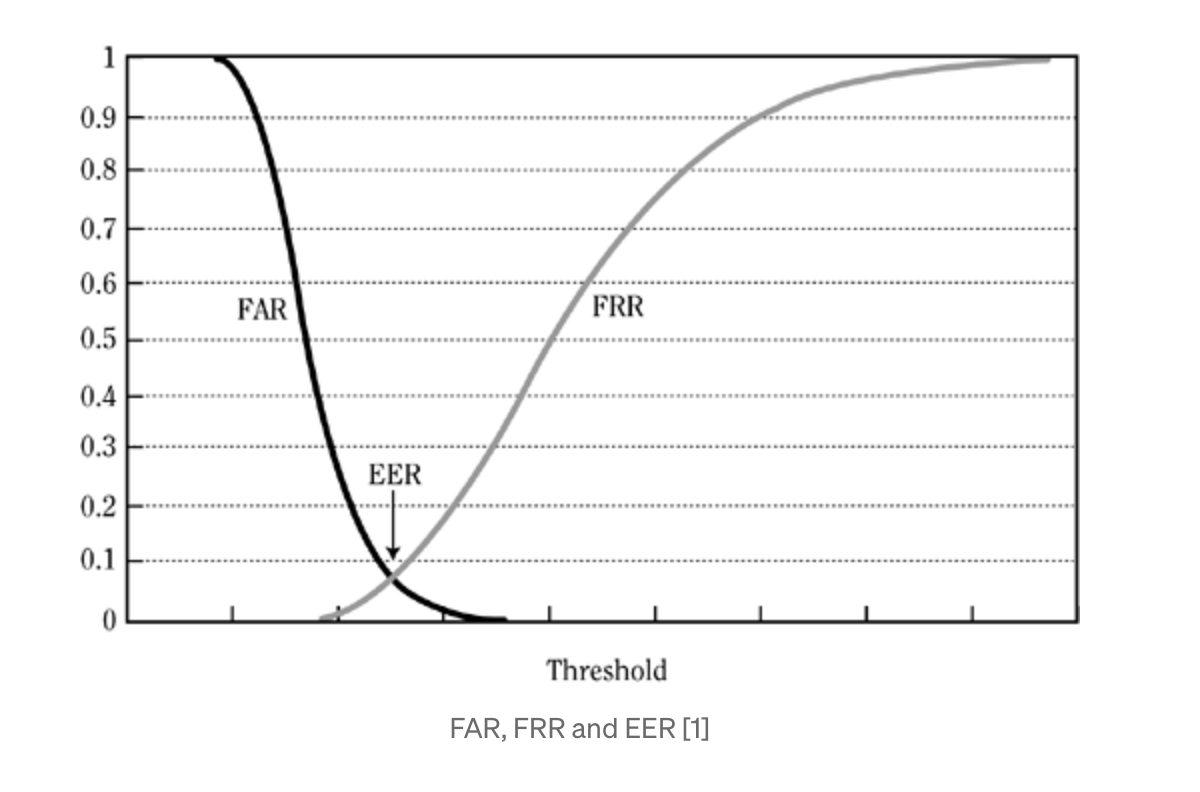
\includegraphics[scale=.5]{images/eer}
            \end{center}
    \end{frame}

\section{Solution}

    \begin{frame}{Sources}
        I relied heavily on
        \begin{itemize}
            \item \href{https://www.kaggle.com/code/awsaf49/asvspoof-2019-tfrecord-data}{https://www.kaggle.com/code/awsaf49/asvspoof-2019-tfrecord-data}
            \item \href{https://www.kaggle.com/code/awsaf49/fake-speech-detection-conformer-tf}{https://www.kaggle.com/code/awsaf49/fake-speech-detection-conformer-tf}
        \end{itemize}
    \end{frame}

    \section{Model}
    \subsection{Data}
    \begin{frame}{Meta Data}
\small

I converted the files to tfrecords

        \begin{itemize}
            \item speaker\_id : LA\_**, a 4-digit speaker ID
            \item filename : LA\_**, name of the audio file
            \item system\_id : ID of the speech spoofing system (A01 - A19), or, for real speech SYSTEM-ID is left blank ('-')
            \item class\_name : bonafide for genuine speech, or, spoof for fake/spoof speech
            \item target : 1 for fake\/spoof and 0 for real/genuine
        \end{itemize}
    \end{frame}



    \subsection{Augmentations Used}
    \begin{frame}
        Audio:
        \begin{itemize}
            \item Random Noise
            \item Random TimeShift
            \item Random CropOrPad
            \item Audio Trim
        \end{itemize}

        Spectogram:
        \begin{itemize}
            \item Random TimeMask
            \item Random FreqMask
            \item CutMix
            \item MixUp
        \end{itemize}
    \end{frame}

    \begin{frame}{Conformer Model}


        \begin{itemize}
            \item The conformer model uses CNN and transformers to combine harvesting global and local features
            \begin{itemize}
            \item Feed-forward module
            \item Self-attention module
            \item Convolution module
            \item Layer normalization module
            \end{itemize}
            \item The backbone used is ImageNet
        \end{itemize}
    \end{frame}
\subsection{Results}
    \begin{frame}{Confusion Matrix}
        \begin{center}
            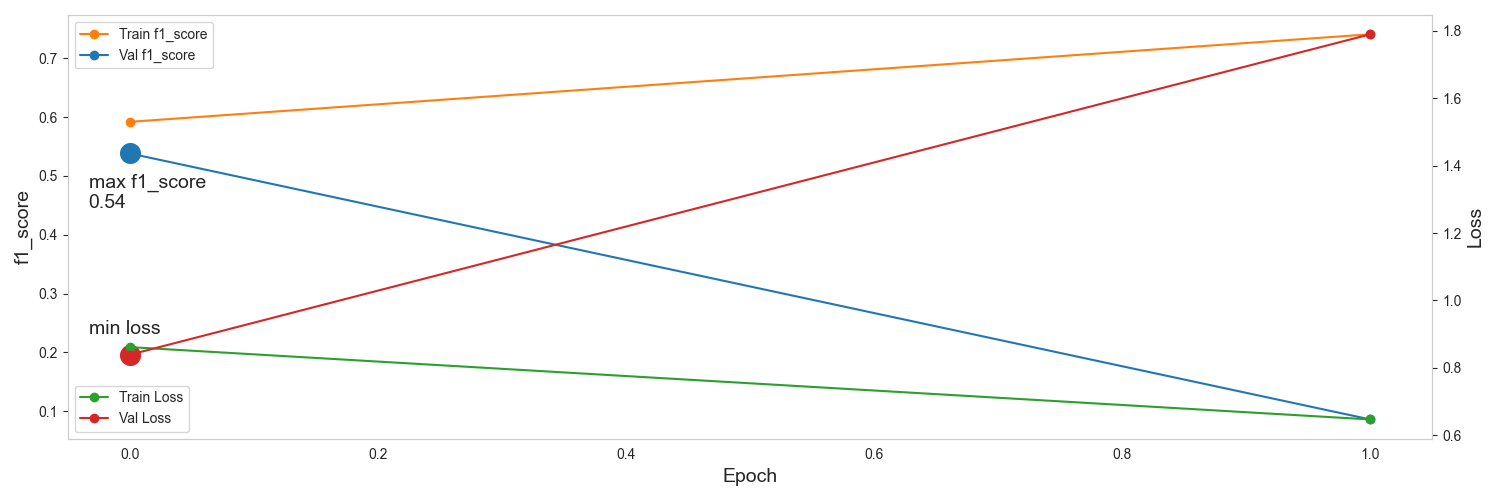
\includegraphics[scale=.4]{images/cm}
        \end{center}
    \end{frame}

    \end{document}



\begin{frame}
    \begin{itemize}
        \item
        \item
    \end{itemize}
\end{frame}




















